\documentclass[a4paper,twoside]{article}

\usepackage{graphicx}
\usepackage{subfigure}
\usepackage{calc}
\usepackage{amssymb}
\usepackage{amstext}
\usepackage{amsmath}
\usepackage{amsthm}
\usepackage{multicol}
\usepackage{pslatex}
\usepackage{apalike}
\usepackage{SCITEPRESS}
\usepackage[small]{caption}
\graphicspath{{images/}}

\subfigtopskip=0pt
\subfigcapskip=0pt
\subfigbottomskip=0pt

\begin{document}

\title{Evaluating Artificial Neural Networks and Traditional Approaches for Risk Analysis in Software Project Management \subtitle{A case study with PERIL dataset} }
\author{\authorname{Carlos H. M. S. Timoteo\sup{1}, Meuser J. S. Valenca\sup{1} and Sergio M. M. Fernandes\sup{1}}
\affiliation{\sup{1}Computer Engineering Department, University of Pernambuco, Rua Benfica, Recife, Brazil}
\email{\{chmst, mjsv, smurilo\}@ecomp.poli.br}
}
%The paper must have at least one keyword. The text must be set to 9-point font size and without the use of bold or italic font style. For more than one keyword, please use a comma as a separator. Keywords must be titlecased.
\keywords{Software Project, Risk Management, Risk Analysis, Support Vector Machine, MultiLayer Perceptron, Monte Carlo Simulation, Linear Regression Model}
%The abstract should summarize the contents of the paper and should contain at least 70 and at most 200 words. The text must be set to 9-point font size.
\abstract{Many software project management end in failure. Risk analysis is an essential process to support project success. There is a growing need for systematic methods to supplement expert judgment in order to increase the accuracy in the prediction of risk likelihood and impact. In this paper, we evaluated support vector machine (SVM), multilayer perceptron (MLP), a linear regression model and monte carlo simulation to perform risk analysis based on PERIL data. We have conducted a statistical experiment to determine which is a more accurate method in risk impact estimation. Our experimental results showed that artificial neural network methods proposed in this study outperformed both linear regression and monte carlo simulation.}

\onecolumn \maketitle \normalsize \vfill

\section{\uppercase{Introduction}}
\label{sec:introduction}
%Apresentar a estatística da quantidade de projetos de software que falham.
\noindent How risky are software projects? Several studies about effectiveness of software cost, scope, schedule estimation techniques; surveys from software professionals in industry; and analysis of project portfolios have been done to answer this question \cite{budzier2013double}. However, there is not a consensus. 

Some authors \cite{schmidt2001identifying} have noticed that many software development projects end in failure. They showed that around twenty five percent of all software projects are canceled outright and as many as eighty percent of all software projects run over their budget, exceeding it by fifty percent in average. Industry surveys suggest that only a quarter of software projects succeed outright, and billions of dollars are lost annually through project failures or projects that do not deliver promised benefits \cite{bannerman2008risk}. Moreover, that study showed evidences that it's a global issue, impacting private and public sector organizations.

%Apresentar a definição de risco (PMBOK). As características do risco de projeto (estocásticos pois levam em consideração o instante atual, podem estar interrelacionados casualmente, a previsão pode ser bem baseada em dados históricos).
Risk can be defined as the possibility of loss or injury \cite{BOEHM1991}. This definition can be expressed by risk exposure formula. This study takes into a definition whereupon project risk is a certain event or condition that, if it occurs, has a positive or negative effect on one or more project objectives \cite{PMBOK2008}. A complement that definition risk is a measure of the probability and severity of adverse effects \cite{haimes2011risk}.

%Páragrafo de ligação para os problemas
%Recent perceptions about risk management and the inherent challenges posed by the nature of software projects contributes to the lack of project stability from majority of software project organizations \cite{kwak2004project}. Those authors have already identified risk management as the least practiced discipline among different project management knowledge areas \cite{kwak2000calculating}. They mention that, probably, a cause for it is that software developers and project managers perceive managing uncertainty processes and activities as extra work and expense.

%Apresentar o problema na análise de risco devido a ausencia de dados históricos em se tratando de projetos. Falta de repetibilidade das atividades. A dificuldade em estimar de forma precisa a probabilidade e o impacto dos riscos.
A limitation can be found in Boehm's risk definition - it is very difficult, in practice, to estimate the probability of many risk factors, especially in software projects \cite{bannerman2008risk}. Probability and impact can only be meaningfully determined for activities that are repeated many times, under controlled circumstances, so the one-off nature of many software project activities mitigates accurate estimates.

%Apresentar o problema da falta de uma ferramenta para suportar gestores que utilizam a intuição ao invés da lógica para analisar o risco.
So, there is an increasing need for more systematic methods and tools to supplement individual knowledge, judgment, and experience. Human traits are often sufficient to address less complex and isolated risks. For example, a portion of the most serious issues encountered in system acquisition are due to ignored risks under low likelihood, until they create serious consequences \cite{higuera1996software}.

%Justificar a escolha dos métodos analisados nesse estudo.
Monte Carlo Simulation (MCS) is cited as a good method for project risk analysis \cite{PMBOK2008}. However, there are some limitations that becomes it unfeasible \cite{Ibbotson2005}. Simulations can lead to misleading result if inappropriate inputs, derived from subjective parametrization, are entered into the model. Commonly, the user should be prepared to make the necessary adjustments if the results that are generated seem out of line. Moreover, Monte Carlo can not model risks correlations. It means that numbers coming out in each draw are random, in consequence, an outcome can vary from its lowest value, in one period, to the highest in the next. Therefore, alternative approaches must be investigated to predict risks.

%Apresentar o objetivo desse trabalho: Analisar qual abordagem é mais eficiente para a análise do impacto do risco no gerenciamento de projetos de software: redes neurais artificiais ou a abordagem tradicional baseada em simulação de monte carlo. Como base de comparação, será utilizada a regressão linear.
The main purpose of this paper is to analyze which is a more efficient approach to software project risk analysis: MCS technique or Artificial Neural Networks (ANN's) alternatives, through Multilayer Perceptron (MLP) and Support Vector Machine (SVM), to improve accuracy and decrease error prone. A Linear Regression Model (LRM) is also considered as baseline during the method.

%Apresentar a metodologia a ser utilizada nesse estudo. Um experimento estatístico para avaliação do erro de previsão do impacto de riscos obtidos a partir da base de dados do PERIL. As quatro técnicas selecionadas nesse estudo irão prever the outcomes to risk impacts, o erro médio absoluto será calculado thirty times, e um teste de hipótese pode ser necessário para afirmar qual a melhor técnica that fits this dataset.
The methodology adopted in this study is a statistical experiment to evaluate the prediction error of risk impact from PERIL dataset \cite{kendrick2003identifying}, a framework to identify risks in software project management. The four selected techniques must estimate the outcome to risk impacts. Mean Absolute Error (MAE) will be calculated thirty times for each approach, and then a hypothesis test may be necessary to achieve the study goal.

%Apresentar as seções seguintes do trabalho.
Section \ref{sec:stateofart} presents basic concepts to perform the experiment. Section \ref{sec:methodology} presents the methodology for this study, including dataset characterization. Section \ref{sec:resultanalysis} presents the result analysis and establishes the best analyzed technique. In the end, Section \ref{sec:conclusion} concludes this work and presents limitations and future works.

\section{\uppercase{State of Art}}
\label{sec:stateofart}

\noindent After a short bibliographic revision, we have identified numerous alternative approaches to risk analysis, which includes Bayesian Belief Networks, Artificial Neural Networks (ANN), Decision Tree (DT), Fuzzy Set Theory (FST), Neuro-Fuzzy System (NFS) \cite{huang2004neuro} \cite{hu2007software} \cite{attarzadeh2010novel} \cite{dzega2010classification} \cite{yu2011software} \cite{saxena2012software} \cite{dan2013improving}.

Genetic algorithm was utilized to improve ANN estimator \cite{hu2007software}. Experimental results showed that it achieved higher accuracy when compared to a SVM model. Moreover, a proposed ANN model that incorporates with Constructive Cost Model (COCOMO) was improved through particle swarm optimization, to estimate the software development effort accurately. Another authors improved cost estimation for COCOMO'81, towards a general framework for software estimation based on NFS \cite{huang2004neuro}.

A model based on fuzzy theory have overcome the difficulty of qualitative and quantitative assessment of traditional methods \cite{yu2011software}. Neuro-fuzzy techniques also was explored to design a suitable model to improve software effort estimation for NASA software projects, on purpose a NFS had the lowest prediction error compared to existing models \cite{saxena2012software}.

Results from risk analysis experiments performed through data mining classifiers - C4.5, RandomTree, classification and regression tree algorithms - have been presented \cite{dzega2010classification}. The authors described how boosting and bagging metaclassifiers were applied to improve the outcomes, but also have analyzed influence of their parameters on generalization and in prediction accuracy. Although, the authors rejected MLP and SVM prematurely.

\subsection{Project Risk Management}

%Apresentar a teoria de gerenciamento de risco de projetos (PMBOK). %O objetivo do gerenciamento de riscos. 
\noindent According to PMI \cite{PMBOK2008}, project risk management includes planning, identification, analysis, response planning, monitoring and controlling risks. Its purpose is to increase likelihood and impact of positive events and reduce probability and severity of negative events. From management point of view, making informed decisions by consciously assessing what can go wrong, as well as its likelihood and severity of the impact, is at the heart of risk management. %This activity involves the evaluation of the trade-offs associated with all policy options for risk mitigation in terms of their costs, benefits, risks and the evaluation of the impact of current decisions on future options.

%O processo de gerenciamento de riscos
Project risk management processes are:
\begin{itemize}
\item Planning risk management: The process of defining how conduct risk management activities;
\item Identifying risks: The process of determining risks that can affect project and documenting its characteristics;
\item Performing qualitative risk analysis: The process of prioritizing risks to analyze through assessment and combination of its occurrence probability and impact;
\item Performing quantitative risk analysis: The process of analyzing numerically the effect of previous identified risks, in terms of general project objectives;
\item Planning risk responses: The process of developing options and actions to increase opportunities and decrease threats to project objetives;
\item Monitoring and controlling risks: The process of implementing risk responses planning, tracking identified risks, monitoring residual risks, identifying new risks and assessing the efficacy of risk treatment process during the whole project.
\end{itemize}

\subsubsection{Risk Analysis}

% Apresentar o conceito de análise de riscos.
\noindent Analysis is the conversion of risk data into risk decision-making information. Analysis provides the basis for the project manager to work on the most critical risks. Boehm (1991) defines risk analysis objective as the assessment of the loss probability and magnitude for each identified risk item, and it assesses compound risks in risk-item interactions. Typical techniques include performance and cost models, network analysis, statistical decision analysis and quality-factor (like reliability, availability, security) analysis.

% Apresentar o processo de análise de riscos. Mostrar que ele é dividido em análise qualitativa e quantitativa.
Risk analysis depends on a good mechanism to identify risks. However, most of the methods assume that managers have the required experience to be aware of all pertinent risk factors, but it can not be the situation. Moreover, many of these methods can be time-consuming and thus too costly to use on a regular basis. Therefore, one popular method for identifying risk factors has been the use of checklists. Unfortunately, these checklists are based in small samples or, even worse, flawed in their risk historical data collection methods.

% Apresentar as técnicas utilizadas no PMBOK para a análise de risco (PRAM)
PMI \cite{PMBOK2008} cites sensibility analysis, earned monetary value (EMV), modeling and simulation, specialized opinion as most used techniques.

\subsubsection{Monte Carlo Simulation}

% Apresentar a definição da simulação de monte carlo.
\noindent Monte Carlo simulation is a technique that computes or iterates the project cost or schedule many times using input values selected at random from probability distributions of possible costs or durations, to calculate a distribution of possible total project cost or completion dates \cite{PMBOK2008}.

A model is developed, and it contains certain input variables. These variables have different possible values, represented by a probability distribution function of the values for each variable. The Monte Carlo method is a detailed simulation approach through intensive computing to determine the likelihood of possible outcomes of a project goal; for example, the completion date. The inputs of the procedure are obtained randomly from specific intervals with probability distribution functions for the durations of schedule activities or items from cost baseline. Those different input values are used to construct a histogram of possible results to the project and its relative probability, but also the cumulative probability to calculate desired contingency reserves for time or cost. Additional results include the relative importance of each input in determining the overall project cost and schedule \cite{kwak2007exploring}.

\subsection{Artificial Neural Networks}

\noindent An ANN is a massively parallel distributed processor made up of simple processing units, which has a natural propensity \cite{haykin1994neural}. It adopts non-parametric regression estimates made up of a number of interconnected processing elements between input and output data.


\subsubsection{MultiLayer Perceptron}

% Apresentar a definição de MLP.
\noindent MLP model is constituted of some neurons organized in at least three layers. The first of them is the input layer, in which input variables are directly connected to a exclusive neuron. The next is the hidden layer that completely connects the neurons from previous layer to the neurons in output layer. Lastly, output layer represents ANN outcome. Each input in a neuron has an associated weight to be adjusted by training algorithm. Common MLP models contain one bias neuron. MLP is a direct graph, in which inputs data are propagated from input layer to hidden layer\(s\) and from hidden layer\(s\) to output layer. The data flow in forward way is known as "forward phase". The data flow in the opposite way is the "backward phase".

One major concern of ANN is the stability-plasticity dilemma. Although continuous learning is desired in ANN, further learning will cause the ANN to lose memory when the weights have reached a steady state \cite{haykin1994neural}. The Backpropagation algorithm is used as training method because it allow us to adjust weights of multilayer networks, towards Generalized Delta Rule \cite{rumelhart1985learning}. 

\subsubsection{Support Vector Machine}

% Apresentar a definição de SVM.
\noindent Support Vector Machine (SVM) is an elegant tool for solving pattern recognition and regression problems. It has attracted a lot of attention from researchers due to its ability to provide excellent generalization performance. The goal of SVM regression is to estimate a function that is as "close" as possible to the target outcomes for every input data in training set and at the same time, is as "flat" as possible for good generalization. More details about SVM can be found in \cite{Shevade1999}.

\section{\uppercase{Methodology}}
\label{sec:methodology}
% Apresentar o objetivo do estudo. Justificar a escolha e a necessidade da base de dados, do pre processamento dos dados, do uso de ferramentas e os experimentos a serem conduzidos.

\noindent In this paper, we analyzed which is a more efficient approach to risk analysis of software projects: MCS, MLP, SVM or a LRM. A LRM was considered as baseline approach. The analysis was made in terms of prediction accuracy. Accuracy means the degree of closeness of a predicted outcome to the true value. A metric of accuracy is the Mean Absolute Error (MAE) given by

\begin{equation}\label{eq_MAE}
    MAE=\frac{1}{n}\sum_{i=1}^{n} |e_i|,
\end{equation}
where $e_i=f_i - y_i$, $f_i$ is the calculated outcome, $y_i$ is the expected outcome and $n$ is the number of data pairs.

The four selected techniques have predicted the outcome to risk impacts. Mean Absolute Error was calculated thirty times for each method. Nevertheless, a Non-paired Wilcoxon Test \cite{siegel1956nonparametric} may be necessary to assert which is a more efficient approach to fit PERIL. Non-paired Wilcoxon Test is used because there were no evidence that the samples came from a normally distributed population, either there were no relation between outcomes from different samples.

One important requirement considered in this study is that the same prediction method must be adopted for each approach. Furthermore, cross-validation \cite{amari1996statistical} must be used to avoid the occurrence of overfitting of data training. For instance, \textit{early stopping} training was used to identify the beginning of overfitting because this method has been proved to be capable of improving the generalization performance of the ANN over exhaustive training \cite{haykin1994neural} \cite{amari1996new}. Therefore, cross-validation method are used for each alternative, excluding Monte Carlo Simulation, to promote higher generalization performance.

\subsection{PERIL Data Set}
\label{sec:perildataset}

%Apresentar a base de dados: Que dados estão presentes? As características dos dados: aleatórios, com viés, não é uma série temporal e não correlação com outros dados.
\noindent A better risk management starts identifying potential problems, asserted here as risk factors. The adoption of available methods like: reviewing lessons learned, brainstorming, interviews and specialized judgment are relative efficient alternatives, otherwise in most of situations it involves high costs. A low cost, extensive and accessible proposal is to use PERIL dataset \cite{kendrick2003identifying}.

For more than a decade, in Risk Management Workshops, Kendrick \cite{kendrick2003identifying} have collected six hundred and forty nine anonymous risk registers from hundreds of project leaders dealing with their past project problems. He has compiled this data in the PERIL database, which summarizes both a description of what went wrong and the amount of impact it had on each project. The dataset provides a sobering perspective on what future projects may face and is valuable in helping to identify at least some of what might otherwise be invisible risks.

In projects, the identified risks can be classified as "known", those anticipated during planning, or "unknown", further identified during project execution. The purpose of this dataset is to provide a framework to identify risks, in such a way to increase the number of "known", and decrease the amount of "unknown" risks.

Some characteristics of PERIL are: 
\begin{itemize}
\item the data are not relational, they contain only most significant risks from tens of thousands projects undertaken by the project leaders from whom they were collected;
\item they present bias, the information was not collected randomly; they are worldwide, with a majority from the Americas and they do not identify opportunities; 
\item the relative impact is based on the number of weeks delayed the project schedule;
\item typical project had a planned duration between six months and one year and typical staffing was rarely larger than about twenty people.
\end{itemize}

Risk registers are categorized as scope, schedule and resource. Scope is decomposed in change and defect subcategories. Schedule is decomposed in dependency, estimative and delay. Resources is decomposed in money, outsourcing and people subcategories. One benefit of PERIL is that the author contemplates black swans - risks with large impact, difficult to predict and with rare occurrence \cite{taleb2001fooled}. 

\subsection{Data Preprocessing}
\label{sec:datapreprocessing}

% O procedimento de pré-processamento dos dados. E a justificativa para os tratamentos realizados nos dados.
\noindent First of all, PERIL contains nominal and numeric values. Nominal variables were expressed through binary variables. In that point, we have utilized twelve binaries variables to represent eight selected nominal variables. Secondly, impact which represents the real output, are integer numbers. We have noticed that impact probability distribution function fits with log-normal and gamma distribution functions. Therefore, we have performed a gamma data normalization \cite{han2006data}. Data preprocessing was suggested by \cite{valenca2005aplicando}.

Figure \ref{fig:input16} and Figure \ref{fig:input712} introduce input variables in histograms. All data are binary values represented by bar graphs, that means the number of occurrences for each value interval. Figure \ref{fig:impacthistogram} presents gamma normalized real outcome from PERIL in a histogram. A shape of the distribution fitting function is also presented in a curve under the histogram. Commonly, the curve under the histogram should seems with normal function graph. Unlikely, we have realized that predicting risk impact from PERIL is not a easy task.

\begin{figure}[!h]
  \vspace{-0.2cm}
  \centering
  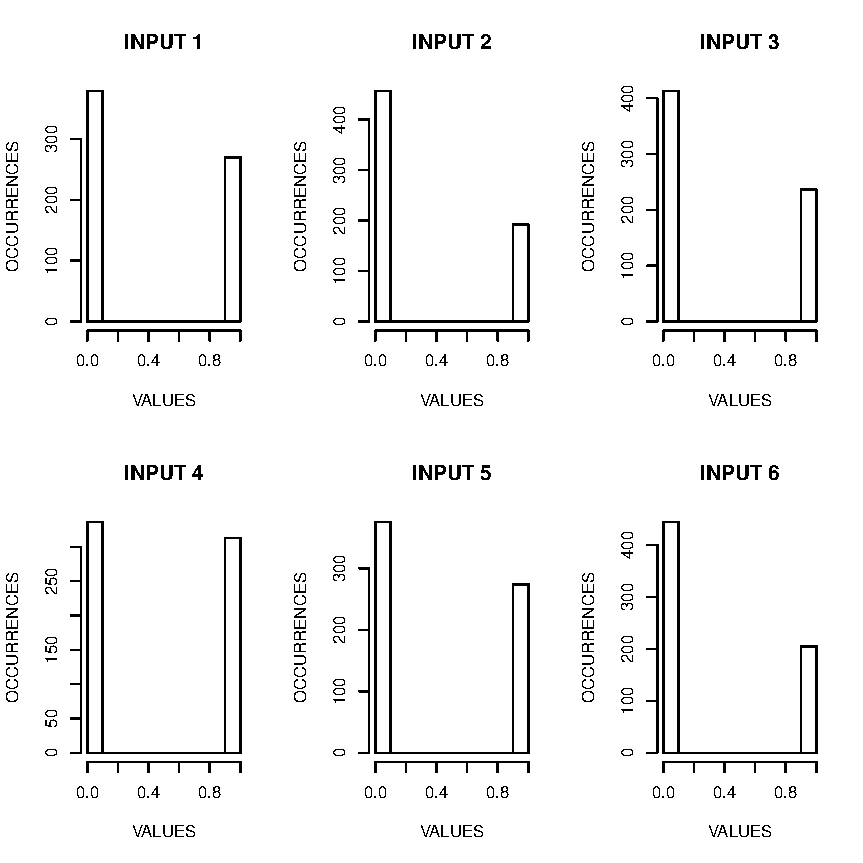
\includegraphics[width=\columnwidth]{images/input1_6.pdf}
  \caption{First six input variables}
  \label{fig:input16}
\end{figure}

\begin{figure}[!h]
  \vspace{-0.2cm}
  \centering
  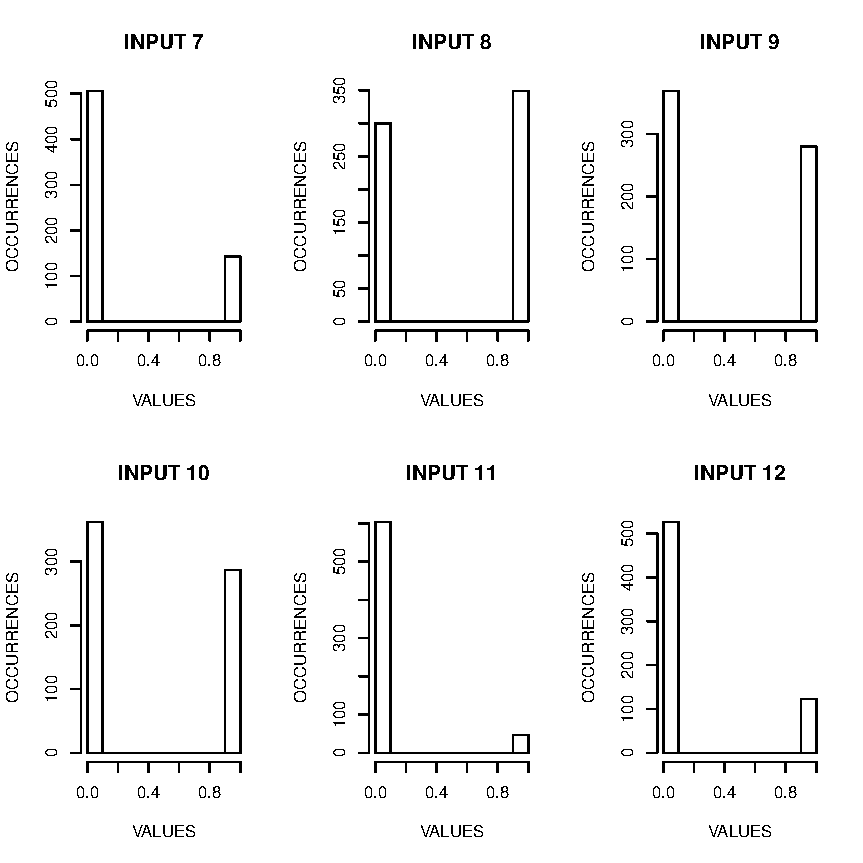
\includegraphics[width=\columnwidth]{images/input7_12.pdf}
  \caption{Last six input variables}
  \label{fig:input712}
\end{figure}

\begin{figure}[!h]
  \vspace{-0.2cm}
  \centering
  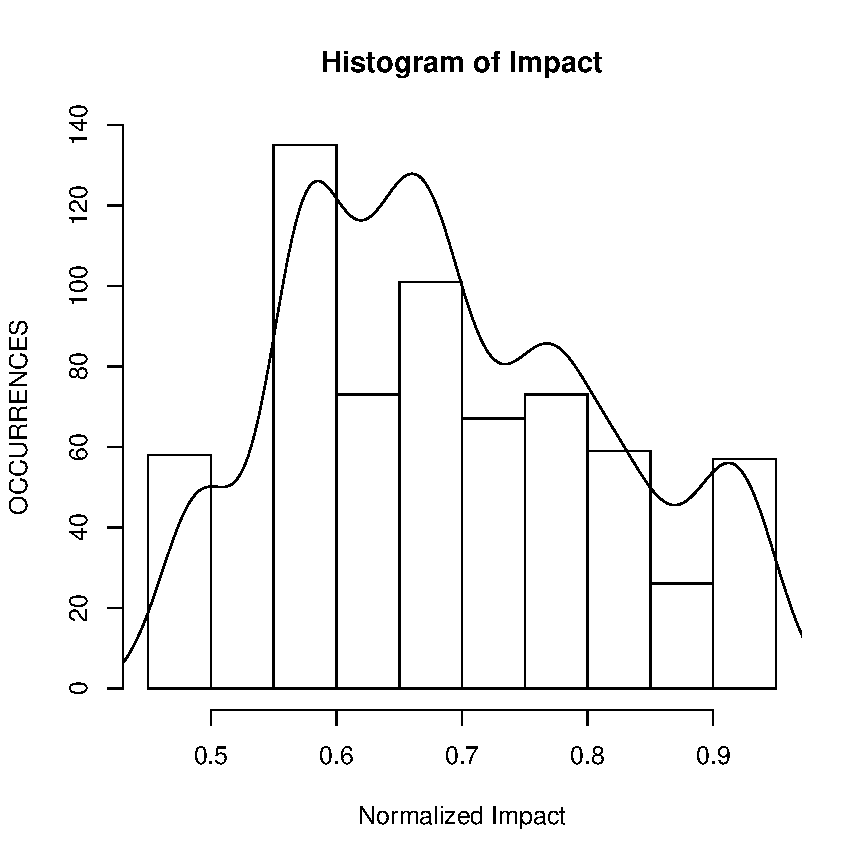
\includegraphics[width=\columnwidth]{images/impact_histogram.pdf}
%  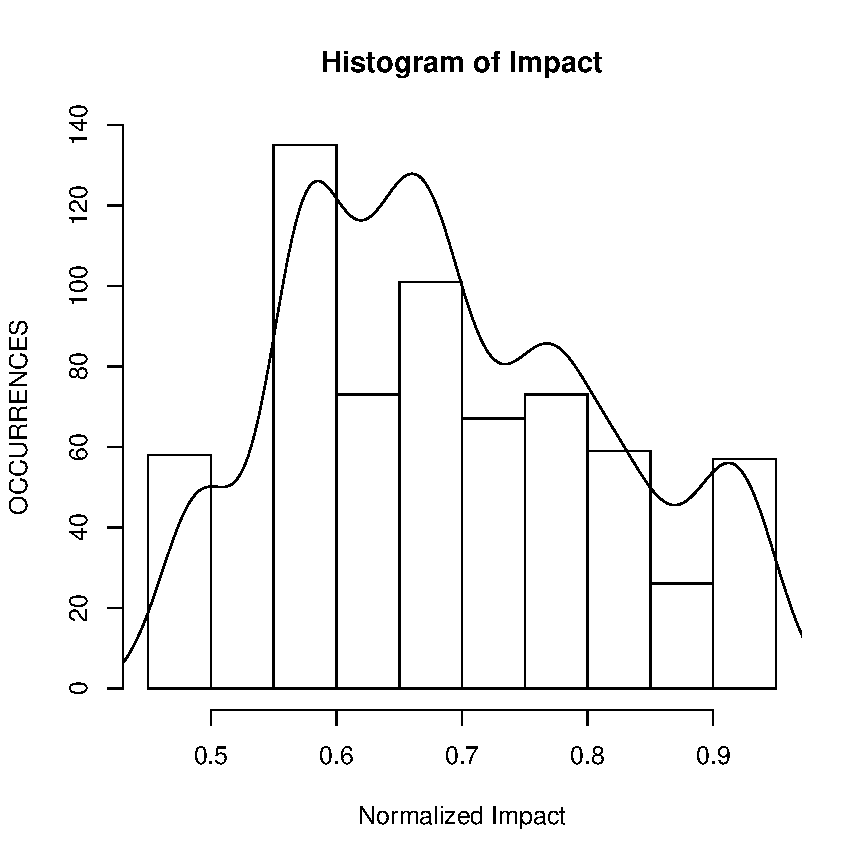
\includegraphics[width=\columnwidth]{images/impact_histogram.pdf}
  \caption{Histogram of impact and shape of the distribution fitting function}
  \label{fig:impacthistogram}
\end{figure}

\subsection{Tools}
\label{sec:tools}

\noindent In sum, we have used several tools during this study. First, MCS was performed in Microsoft Office Excel, we have utilized Data Analysis complement to obtain random values from customized sample. Second, R software was utilized to conduct a experiment with Multiple Linear Regression (MLR) and Regression Tree Model (RTM). R is also a programming language for statistical computing, data manipulation, calculation and graphical display \cite{venables2002introduction}. Third, MLP model was developed in Java. The source code implements data preprocessing, training, cross-validation, testing and MAE evaluation. It was based on \cite{valenca2005aplicando} book. Finally, we have utilized WEKA API \cite{hall2009weka} to program SVM. The built-in implementation of SVM is SMOreg \cite{Smola1998}. The authors proposed an iterative algorithm, called sequential minimal optimization (SMO), to solve the regression problem using SVM. SMOreg, a SMO program, come across our needs because the regression model could be generated after testing and cross-validation as stopping criteria.
% Apresentar a ferramenta Weka e como elas foram configuradas.
%The Waikato Environment for Knowledge Analysis (WEKA) \cite{hall2009weka} came about through the perceived need for a unified workbench that would allow researchers easy access to state of the art techniques in machine learning. WEKA project allows users to quickly try out and compare different machine learning methods on new datasets. Its modular and extensible architecture allows sophisticated data mining processes to be built up from the wide collection of base learning algorithms and tools provided. Extend the toolkit is easy because of a simple API, plugin mechanisms and facilities that automate the integration of new learning algorithms with WEKA’s graphical user interfaces \cite{hall2009weka}.

\subsection{Experiment}
\label{sec:experiment}

\noindent For our purpose, PERIL was split into three disjoint subsets - training, cross-validation and test subsets, corresponding to fifty, twenty-five and twenty five percent of the dataset, respectively. \textit{Split-sample} cross-validation method was used for MLRM and RTM models. Whereas \textit{early stopping} and \textit{split-sample} cross-validation methods were combined and used for MLP and SVM training \cite{priddy2005artificial}.

% Descrever os parâmetros de cada algoritmo utilizado.
MCS technique used the entire dataset. In order to increase the performance prediction, we have filtered only the possible real outcomes to generate the calculated outcome. Towards this decision, we have reduced prediction issues and have improved its performance.

The source code of MLR model was adapted from Torgo \cite{torgo2003data} in order to perform linear regression model training, cross-validation, outcome prediction and MAE evaluation. MLR and RTM models were analyzed statistically to define the baseline linear regression model for further analysis. The results are presented in Section \ref{sec:resultanalysis}.

% Descrever os parametros da MLP
A three layered back-propagation MLP model was established to model risk impact predictor. That model consists of one input layer, one hidden layer, and one output layer. The input layer had thirteen neurons, which represent the twelve independent variables plus the bias. The output layer has one neuron, which represents the single impact outcome. The transfer function in hidden and output layer was sigmoid-logistic. The architecture of the MLP is demonstrated in Figure \ref{fig:mlpmodelstudy}.

\begin{figure}[!h]
  \vspace{-0.2cm}
  \centering
  \def \svgwidth{0.85\columnwidth}
  \input{images/mlp.pdf_tex}
  \caption{MLP model utilized in the study.}
  \label{fig:mlpmodelstudy}
\end{figure} 

The number of neurons in the hidden layer and other paramenters were determined by trial and error, a fast approach aiming to achieve a more accurate performance of MLP. For the analysis, the maximum training epochs has been set at six hundreds. Starting with one neuron in the hidden layer, the MLP model was trained and tested. At each time, the number of neurons was increased by one, until reach ten, from then the number of neurons was increased by ten, until reach one hundred. Learning rate and momentum were increased by 0.1, varying from 0.1 to 0.9. 

Learning rate, momentum and neurons in hidden layer varied from values presented in Table \ref{tab:mlp_configuration_investigation}. A better parameters configuration solution is shown in Table \ref{tab:mlp_best_configuration}. Figure \ref{fig:mlpmodelstudy} presents MLP model with the better configuration for PERIL. The model contains ten neurons in hidden layer.

\begin{table}[h]
\caption{Parameters intervals to MLP model.}\label{tab:mlp_configuration_investigation} \centering
\begin{tabular}{|c|c|c|}
  \hline
  Parameter & Min. Value & Max. Value \\
  \hline
  Momentum & 0.5 & 0.9 \\
  \hline
  Learning rate & 0.1 & 0.5 \\
  \hline
  Hidden Neurons & 1 & 100 \\
  \hline
\end{tabular}
\end{table}

\begin{table}[h]
\caption{A better parameters configuration to MLP model.}\label{tab:mlp_best_configuration} \centering
\begin{tabular}{|c|c|}
  \hline
  Parameter & Value \\
  \hline
  Momentum & 0.5 \\
  \hline
  Learning rate & 0.1 \\
  \hline
  Hidden Neurons & 10 \\
  \hline
  Maximum Cycles & 600 \\
  \hline
\end{tabular}
\end{table}

% Descrever a SVM utilizada e seus parâmetros
In SVM source code, RegSMOImproved class contains optimization algorithm method and PolyKernel was the kernel function described in \cite{Shevade1999}. Other parameters were set in default.

\section{\uppercase{Result Analysis}}
\label{sec:resultanalysis}

%Apresentar os resultados lado a lado para cada algoritmo:
% 1. Apresentar a estatística descritiva para os resultados obtidos dos experimentos (esperado e o obtido).
% 2. Apresentar o erro médio absoluto para as estimatívas.
\noindent Initially, the previous analysis consisted of choosing between MLRM and RTM as baseline approach. It could be performed after discussing the information provided in Table \ref{tab:lm_descriptive} and in Figure \ref{fig:mlrm_result}. 

Table \ref{tab:lm_descriptive} shows descriptive statistics of normalized MAE's to both algorithms. Mean, standard deviation, minimum and maximum value are calculated for MLRM (cv.lm.v1), $RTM_1$ (cv.rpart.v1), $RTM_2$ (cv.rpart.v2) and $RTM_3$ (cv.rpart.v3). $RTM_1$, $RTM_2$ and $RTM_3$ are regression tree models instances automatically generated by R in this analysis. The first method had lower values in all statistics.

\begin{table}[h]
\caption{Descriptive statistics for normalized errors of linear regression models.}\label{tab:lm_descriptive} \centering
\begin{tabular}{|c|c|c|c|c|}
  \hline
   & MLRM & $RTM_1$ & $RTM_2$ & $RTM_3$ \\
  \hline
  Mean & \textbf{0.09912} & 0.10238 & 0.10305 & 0.10361  \\
  \hline
  Std Dev & \textbf{0.00391} & 0.00423 & 0.00441 & 0.00426  \\
  \hline
  Min. & \textbf{0.08956} & 0.09214 & 0.09321 & 0.09372  \\
  \hline
  Max. & \textbf{0.10746} & 0.11231 & 0.11267 & 0.11359  \\
  \hline
\end{tabular}
\end{table}

In Figure \ref{fig:mlrm_result}, normalized MAE's boxplots after predictions for $RTM_3$, $RTM_2$, $RTM_1$ and MLRM are presented. The last boxplot, placed more in the left was obtained to MLRM. 

We could realize that MLRM is a more efficient and precise model and will be introduced in the experiment as baseline method. It is justifiable because that model showed lesser MAE's, minor average/ standard deviation/ minimum/ maximum values and a more parsimonious model compared with RTM.

\begin{figure}[!h]
  \vspace{-0.2cm}
  \centering
  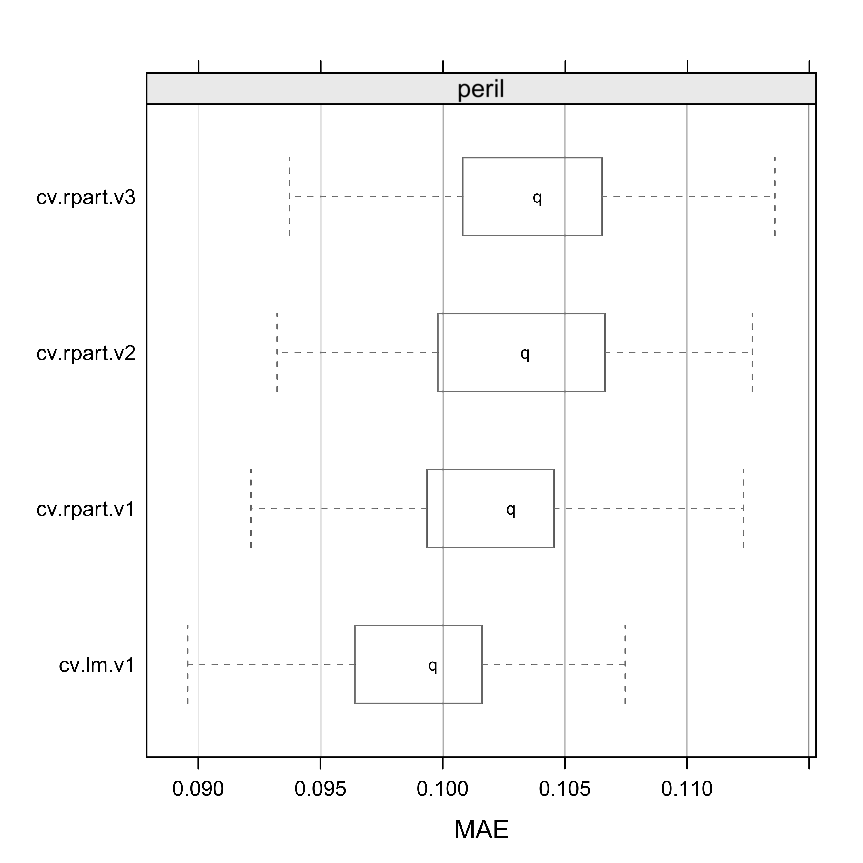
\includegraphics[width=\columnwidth]{images/mlrm_result_peril.pdf}
  \caption{Boxplots for normalized errors of linear regression models.}
  \label{fig:mlrm_result}
\end{figure}

After that, we could perform the main analysis in this paper. Table \ref{tab:final_descriptive} shows descriptive statistics of normalized MAE's for ANN's (SVM and MLP), MLR and MCS. It was perceived that SVM had lower values for minimum (Min.), median, mean and maximum (Max.) errors. Nevertheless, MLP had minor standard deviation (Std.) value.

In Figure \ref{fig:final_result}, it is observed that the traditional technique, MCS (monte carlo simulation), had a large standard deviation. It is due to randomness in MCS method, one of its limitation. Besides that, MCS had higher statistics. On the other hand, comparing MCS with MLR it is noticed that MLR had better statistics. Thus, for this study, we could not identify a reason to justify MCS usage for risk analysis, proposed by \cite{PMBOK2008}. That was one of our premises.

Besides that, MLP seemed to be a promising alternative because it is like a optimized MLR, because MLP is a universal approximator of nonlinear functions and its efficiency was proven in the most different application areas. In this study, MLP was a more precise method to risk impact estimation.

Commonly, SVM has a higher generalization capability, which means 1.5\% better results compared with MLP, approximately \cite{haykin1994neural}. That is because SVM can distinguish small subsets in training data. However, it requires a long training time due to its complexity.

Therefore, accordingly with this study, SVM seems to be a more accurate method to risk impact estimation using PERIL. We can conclude that because it explored a lesser MAE and had a good generalization capability, since its inter-quartil interval was the second shorter, according to Figure \ref{fig:final_result}. But above all, SVM could explore MAE optimization problem. We can realize it observing Figure \ref{fig:svm_exclusive}, in which the most of values are near and above median value.

\begin{table}[h]
\caption{Descriptive statistics for SVM, MLP, MLR and MCS.}\label{tab:final_descriptive} \centering
\begin{tabular}{|c|c|c|c|c|}
  \hline
   & SVM & MLP & MLR & MCS \\
  \hline
  Min. & \textbf{0.08347} & 0.09736 & 0.09764 & 0.10410  \\
  \hline
  Median & \textbf{0.09374} & 0.10014 & 0.10798 & 0.12740 \\
  \hline
  Mean & \textbf{0.09430} & 0.10005 & 0.10798 & 0.12640 \\
  \hline
  Std. & 0.00488 & \textbf{0.00154} & 0.00794 & 0.01250 \\
  \hline
  Max. & \textbf{0.10284} & 0.10413 & 0.12927 & 0.14950 \\
  \hline
\end{tabular}
\end{table}

\begin{figure}[!h]
  \vspace{-0.2cm}
  \centering
  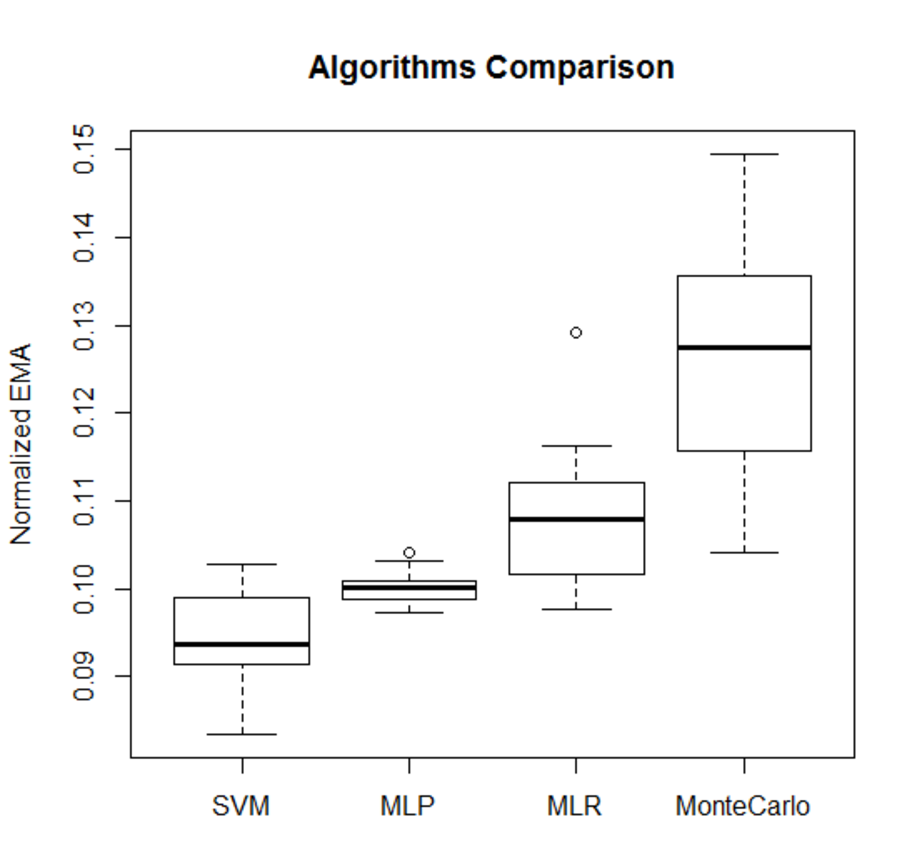
\includegraphics[width=\columnwidth]{images/resul_final.pdf}
  \caption{Boxplots of analyzed methods.}
  \label{fig:final_result}
\end{figure}

\begin{figure}[!h]
  \vspace{-0.2cm}
  \centering
  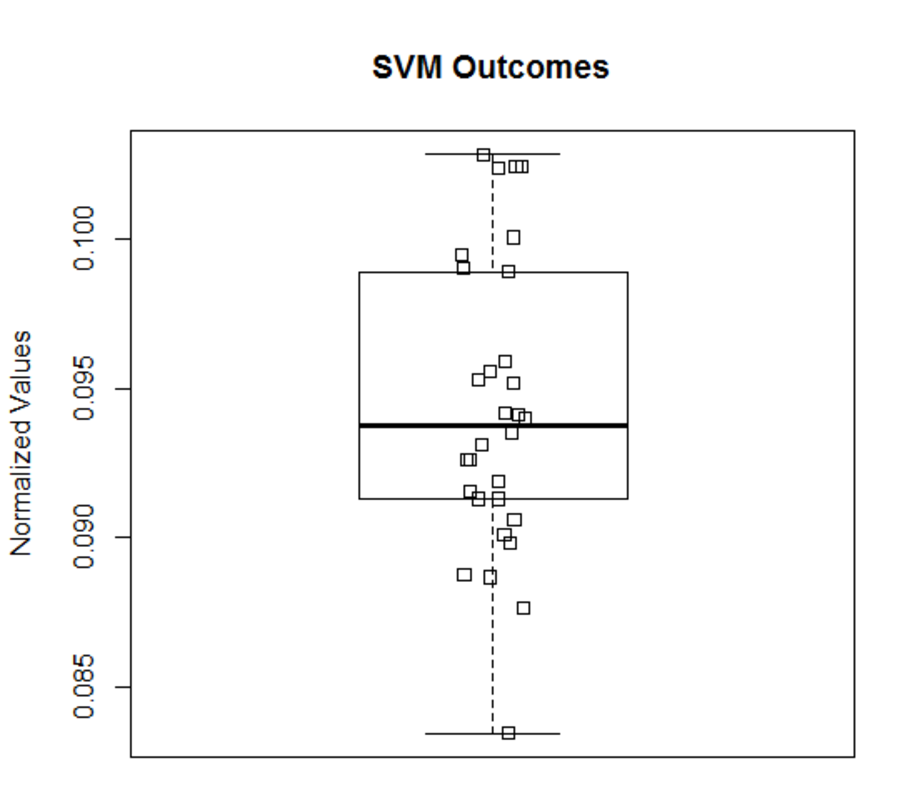
\includegraphics[width=\columnwidth]{images/svm_exclusive.pdf}
  \caption{SVM boxplot with individual values.}
  \label{fig:svm_exclusive}
\end{figure}

\section{\uppercase{Conclusion}}
\label{sec:conclusion}

\noindent This paper has investigated the use of artificial neural networks algorithms, like SVM and MLP, for estimation of risk impact in software project risk analysis. We have carried out a statistical analysis using PERIL. The results were compared to MLRM and Monte Carlo Simulation, a traditional approach proposed by \cite{PMBOK2008}. We have considered improving risk impact estimation accuracy during software project management, in terms of MAE mean and standard deviation. We have observed that MLP had minor standard deviation estimation error, and showed to be a promissory technique. Moreover, SVM had minor estimation error outcomes using PERIL, which a more accurate method. Therefore, the selected ANN algorithms outperformed both linear regression and MCS. Future works should analyze another ANN models and MLP training methods.
% Apresentar os melhores resultados obtidos.
% Apresentar as limitações desse estudo e trabalhos futuros.

\bibliographystyle{apalike}
{\small
\bibliography{example}}
%\section*{\uppercase{Appendix}}
%\noindent If any, the appendix should appear directly after the
%references without numbering, and not on a new page. To do so please use the following command:
%\textit{$\backslash$section*\{APPENDIX\}}

\vfill

\end{document}

